\section{Iteración I}
\subsection{Resumen}
En esta iteración se realizó el renderizado de un modelo 3d propio, así como implementarlo en la aplicación.
\subsection{Desarrollo}
El renderizado de un modelo 3d se a realizo utilizando la herramienta blender, es dicha herramientas modelamos una simple capsula, que se exporto en dos tipos de archivos .obj y .mtl los cuales convertimos, usando Google Sceneform Tools, en un modelo entendible para ARcore.
\begin{figure}[H]
	\centering
	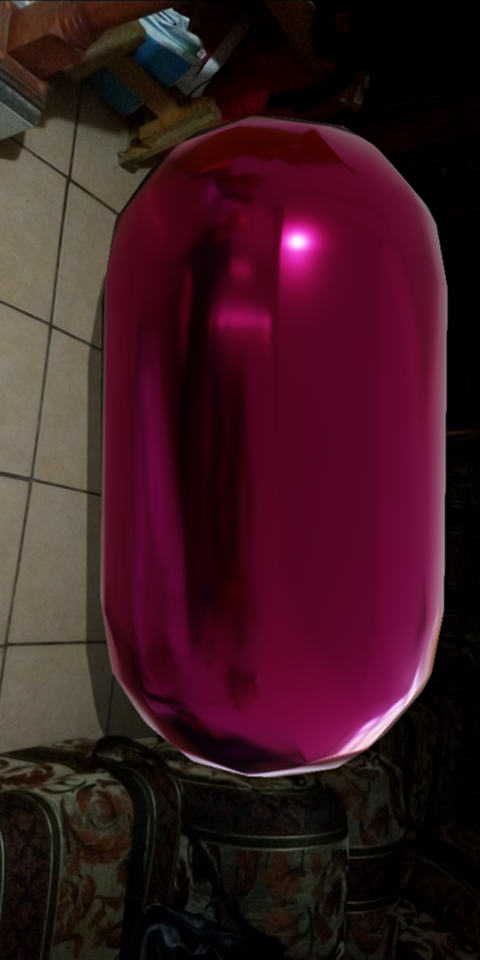
\includegraphics[width=8cm,height=12cm]{imagenes/iteraciones/AR2.png}
	\caption{Primer modelo 3D implementado en ARcore}
	\label{fig:1modelo}
\end{figure} 